\documentclass[a4paper]{report} % set paper size

\usepackage[utf8]{inputenc}
\usepackage {url}
\usepackage[top=2.54cm, bottom=2.54cm, left=2.54cm, right=2.54cm]{geometry} % set margin
\usepackage{amsfonts} % for set names
\usepackage{amsmath} % for equation system
\usepackage{amsthm} % for theorem block
\usepackage{fixltx2e} % for subscript
\usepackage{fancyhdr} % for footer/headline modification
\usepackage{xcolor}
\usepackage{graphicx} % for image insertion
\usepackage[ruled,vlined]{algorithm2e} % for algorithm integration

\pagestyle{fancyplain} % for footing modification on all pages
\fancyhf{}
%\renewcommand{\headrulewidth}{0pt} % remove decorative lign
\fancyhead[L]{Alexandre Devienne EL BA1 2014}
\fancyhead[R]{EPFL}

\begin{document}

\section*{Autumn programming project : Recolor}
The program's organisation is as follows :
\begin{enumerate}
\item Read the inputs

The entire input (image's pixel excepted) is divided into 3 functions which read a specific chunk (i.e.: all threshold together).
These functions dynamically allocate memory for the tables which are freed in main at the end of program.

\item Process the inputs
    \begin{enumerate}
    \item Read the image's pixels
    \item Convert the image into greyscale and compare it to the thresholds
    \item Filter image
    \end{enumerate}
\item Print the output (a single function does this job)
\end{enumerate}

To furthermore show the abstraction made using function in this program we can consider the very basic functions : set\_border, copy\_2D\_tab and reset\_voisin.
Even though they are only called once in the program they 

re-utilisation :
dichotomie like search for seuillage
dynamic memory allocation for matrix and tables (even checks if the allocation is sucesful)

show abstraction/re-usage of fct
One particular thing to note is that my seuillage function is based on dicotomie search

%Complexity of filtrage
%set border : 2 + 2nbC + 2 nbL
%1 + nbF * (nbL * nbC * (6+1 + 9 * 9+ 2) + nbC*nbL)
%tot = nbF*nbC*nbL (90)


\begin{algorithm}
    \KwData{$image$ that went through the threshold, $nbF$ number of filter}
    \KwResult{Filtered $image$}
    \BlankLine
    Let $temp$ be an image which as the original $image$'s size\;
    Let $T$ be a table of colors which can store $3$ entries with each a parameter named $amount$\;

    \BlankLine
    Set the border of $temp$ to black\;
    \For{$i \leftarrow 1$ \KwTo $nbF$}{
        \For{each $pixel$ in $image$ (border excepted)}{
            $resultColor \leftarrow $ NULL\;
            Reset $T$ (remove all entries)\;
            \For{each $neighbor$ of $pixel$} {
                \If{$resultColor = $ NULL} {
                    $resultColor \leftarrow $ \emph{insertInTable}($neighbor$, $T$)\; 
                }
            }
            \If{$resultColor = $ NULL} {
                $resultColor \leftarrow$ black \;
            }
            Set corresponding $pixel$ of $temp$ to $resultColor$\; 
        }
        $image \leftarrow temp$\;
    }

\BlankLine
\SetKwProg{Fn}{Function}{}{}
\Fn{insertInTable($color$, $T$)}
{
\KwIn{$color$ to insert in table $T$ (limited size, a parameter named $amount$ for each entry)}
\KwOut{Color of the pixel after the filter step, or NULL if cannot decide yet}
\BlankLine
\uIf{$color$ already in $T$} {
    Increment corresponding $amount$ by 1\;
    \If{$amount \ge 6$} {
        \KwRet $color$
    }
}
\uElseIf{$T$ full} {
    \KwRet black\;
}
\Else
{
    Store $color$ in new entry of $T$\;
    Set correponding $amount$ to 1\;
}
\KwRet NULL
}
\caption{Filter algorithm}
\end{algorithm}

\begin{figure}
\begin{center}
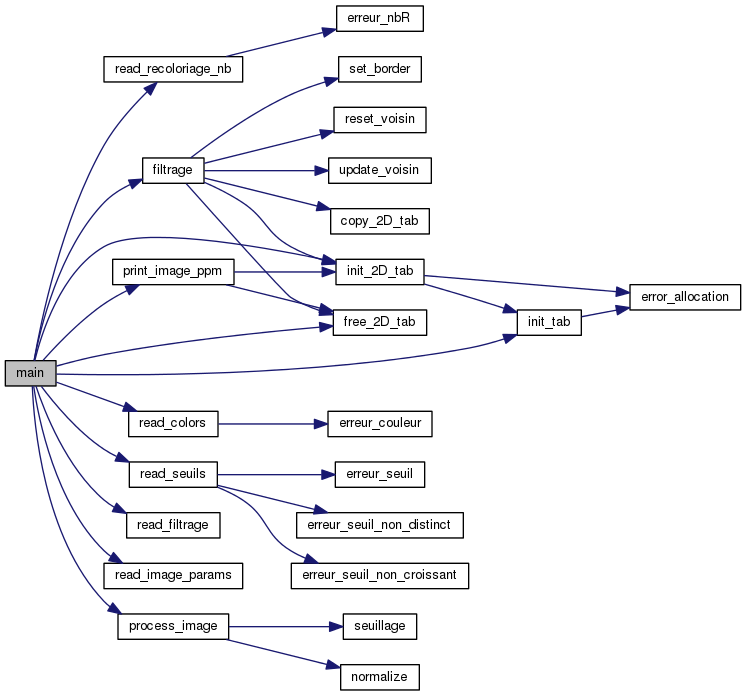
\includegraphics[scale=0.6]{graph.png}
\end{center}
\caption{Call graph}
\end{figure}

\end{document}
